\documentclass{article}

\usepackage{graphicx}
\usepackage{tikz}
\usepackage{tikzsymbols}
\usetikzlibrary{calc,patterns,shapes.geometric}
\pagestyle{empty}
\usepackage[margin=0pt]{geometry}
\geometry{papersize={14in,12in}}

\def\centerarc[#1](#2)(#3:#4:#5){\draw[#1] ($(#2)+({#5*cos(#3)},{#5*sin(#3)})$) arc (#3:#4:#5);}

\begin{document}
	\begin{figure}
		\centering
		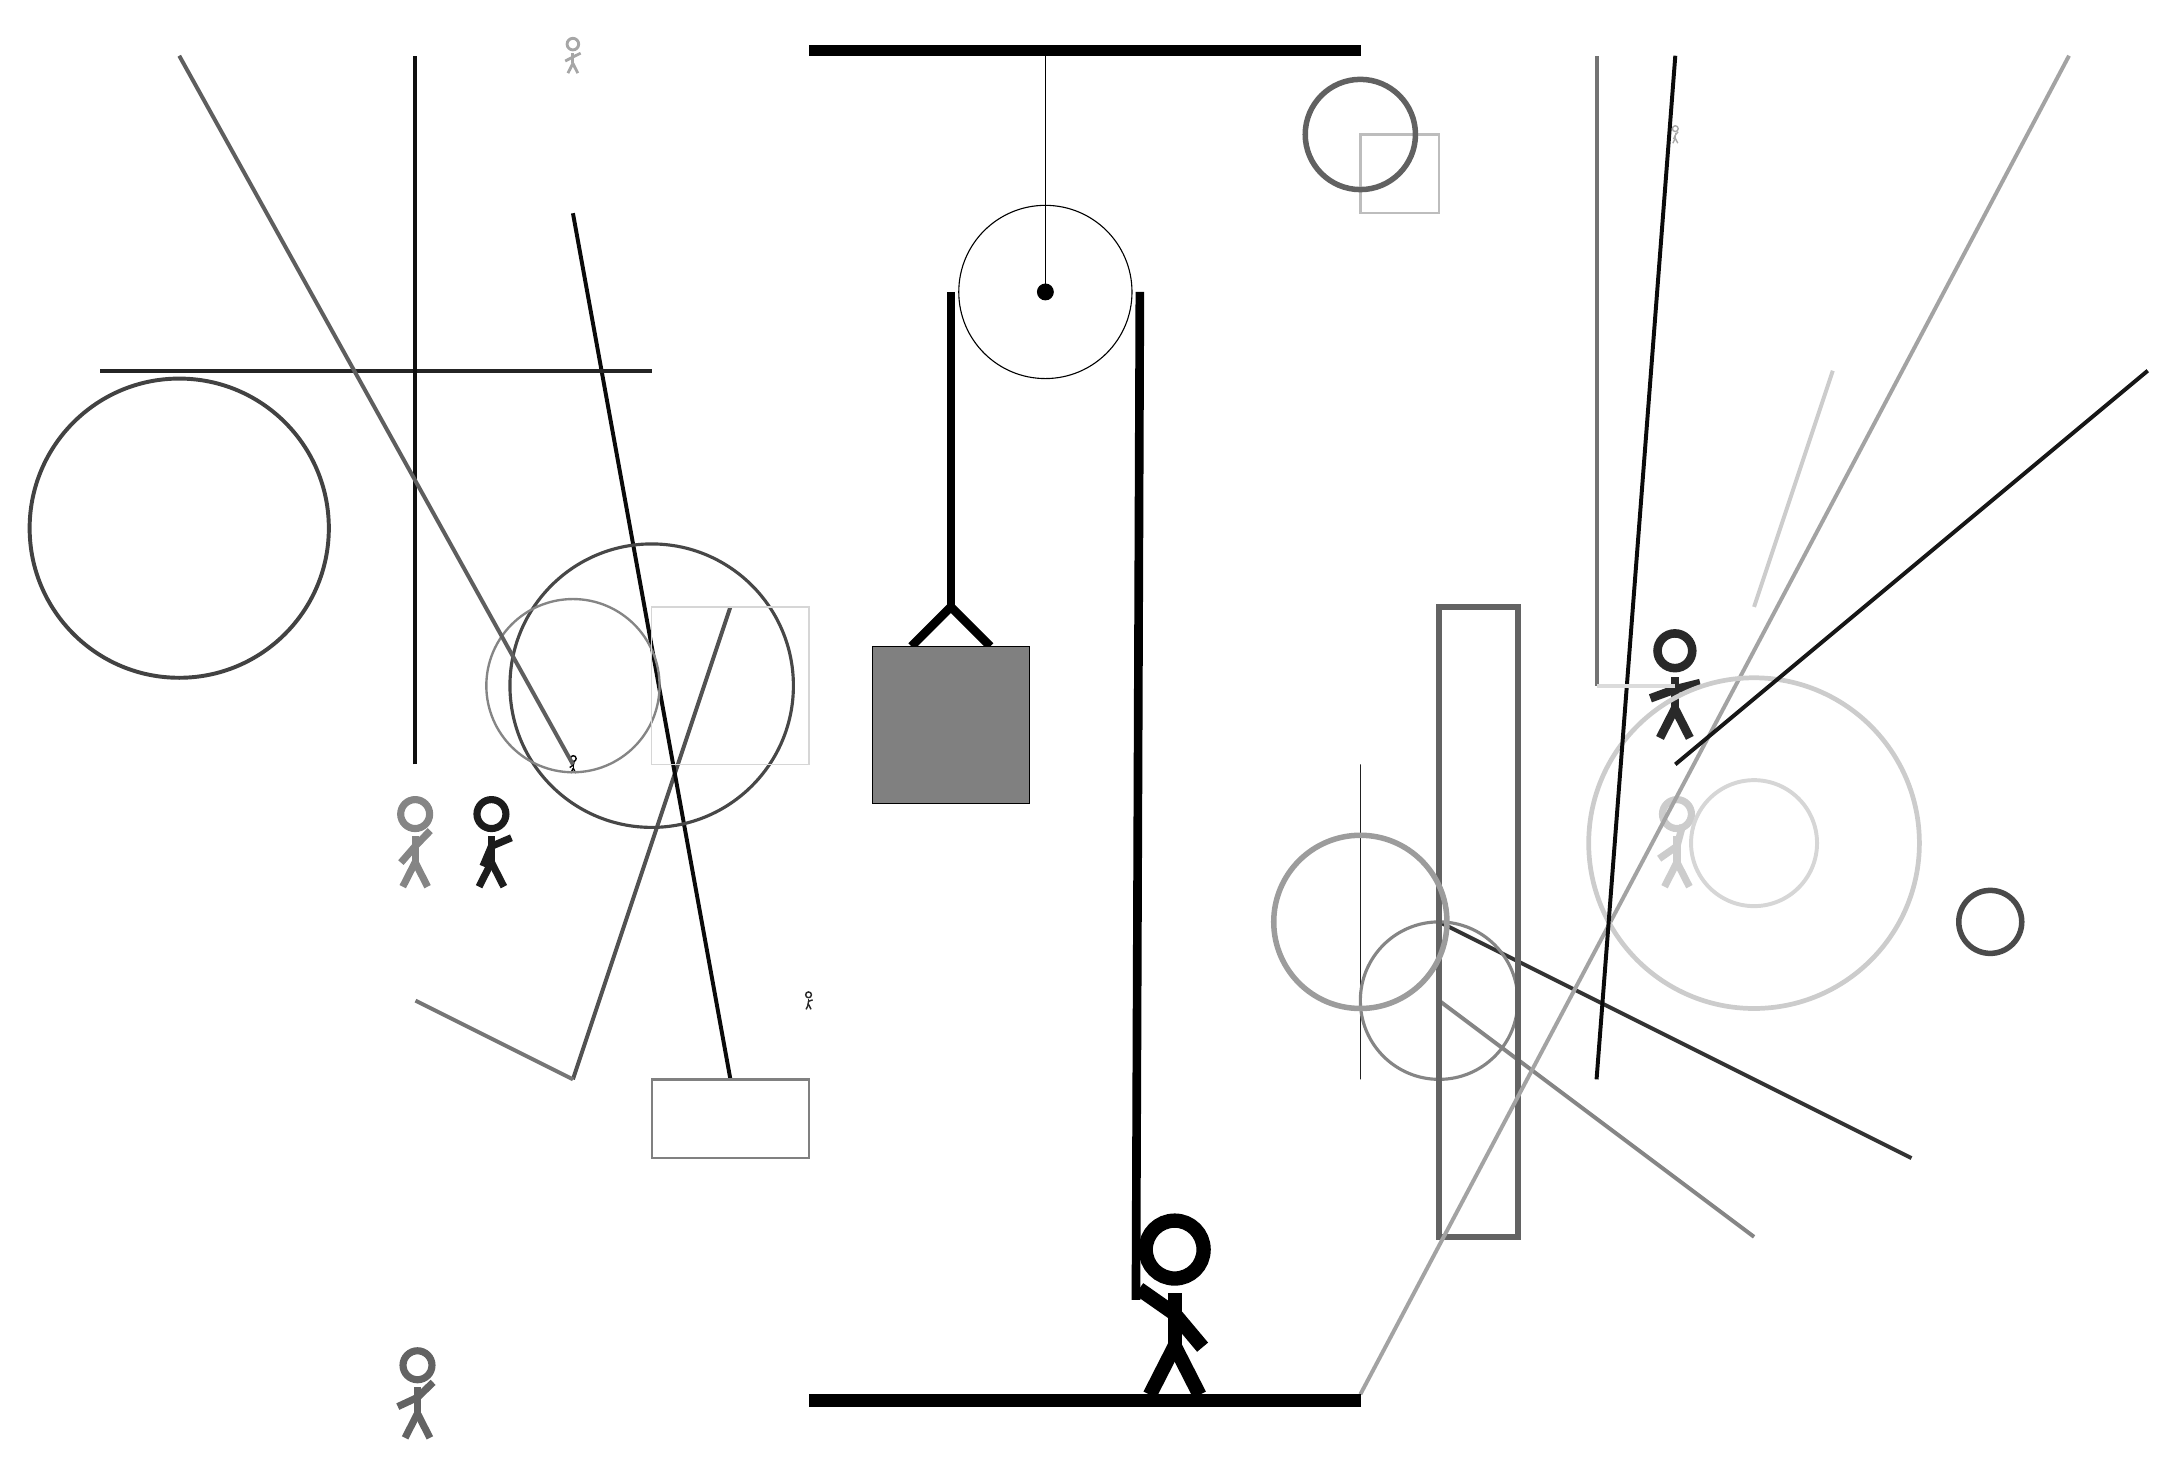
\begin{tikzpicture}
			%%%%% START %%%%%
			
			\draw[fill=black] (-2, 14) rectangle (5, 14.125);
			
			\draw (1, 11) circle (1.1);
			\draw[fill=black] (1, 11) circle (0.1);
			\draw (1, 14) -- (1, 11);
			
			\draw[line width=1.1mm] (-0.7, 6.5) -- (-0.2, 7.0) -- (0.3, 6.5);
			\draw[fill=black!50] (-1.2, 6.5) rectangle (0.8, 4.5);
			
			\draw[line width=0.5mm, color=black!55](8, 6) -- (8, 14);
			
			\draw[line width=0.5mm, color=black!48](10, -1) -- (6, 2);
			\draw[line width=0.5mm, color=black!68](-5, 1) -- (-3, 7);
			\node[line width=0.2mm, color=black!84] at (9, 6) {\Strichmaxerl[6][20][14]};
			
			\node[line width=0.5mm, color=black!20] at (9, 4) {\Strichmaxerl[5][35][75]};
			\draw[line width=0.5mm, color=black!80](6, 3) -- (12, 0);
			\draw[line width=0.2mm, color=black!87] (5, 1) rectangle (5, 5);
			
			\draw [line width=0.5mm, color=black!74](-10, 8) circle (1.9);
			\draw [line width=0.4mm, color=black!48](6, 2) circle (1.0);
			\draw [line width=0.5mm, color=black!16](10, 4) circle (0.8);
			
			\node[line width=0.7mm, color=black!89] at (-6, 4) {\Strichmaxerl[5][67][23]};
			\draw[line width=0.5mm, color=black!96](-5, 12) -- (-3, 1);
			\draw[line width=0.3mm, color=black!26] (6, 12) rectangle (5, 13);
			
			\draw[line width=0.7mm, color=black!61] (7, -1) rectangle (6, 7);
			\draw[line width=0.5mm, color=black!54](-5, 1) -- (-7, 2);
			\node[line width=0.6mm, color=black!48] at (-7, 4) {\Strichmaxerl[5][49][46]};
			
			\draw[line width=0.5mm, color=black!20](10, 7) -- (11, 10);
			\draw[line width=0.5mm, color=black!36](5, -3) -- (14, 14);
			\draw [line width=0.7mm, color=black!62](5, 13) circle (0.7);
			
			\node[line width=0.7mm, color=black!35] at (-5, 14) {\Strichmaxerl[2][28][26]};
			\node[line width=0.6mm, color=black!34] at (9, 13) {\Strichmaxerl[1][67][51]};
			
			\draw [line width=0.7mm, color=black!71](13, 3) circle (0.4);
			
			\draw [line width=0.6mm, color=black!20](10, 4) circle (2.1);
			\draw[line width=0.3mm, color=black!50] (-4, 0) rectangle (-2, 1);
			\draw [line width=0.7mm, color=black!39](5, 3) circle (1.1);
			\draw [line width=0.4mm, color=black!72](-4, 6) circle (1.8);
			
			\node[line width=0.2mm, color=black!98] at (-5, 5) {\Strichmaxerl[1][35][77]};
			\node[line width=0.4mm, color=black!61] at (-7, -3) {\Strichmaxerl[5][25][44]};
			
			\draw [line width=0.3mm, color=black!48](-5, 6) circle (1.1);
			\draw[line width=0.5mm, color=black!86](-4, 10) -- (-11, 10);
			\draw[line width=0.5mm, color=black!91](9, 5) -- (15, 10);
			
			\draw[line width=0.5mm, color=black!94](-7, 5) -- (-7, 14);
			\node[line width=0.3mm, color=black!84] at (-2, 2) {\Strichmaxerl[1][80][18]};
			
			\draw[line width=0.5mm, color=black!96](9, 14) -- (8, 1);
			\draw[line width=0.5mm, color=black!63](-5, 5) -- (-10, 14);
			\draw[line width=0.5mm, color=black!14](9, 6) -- (8, 6);
			\draw[line width=0.2mm, color=black!16] (-2, 7) rectangle (-4, 5);
			
			\draw[line width=1.1mm] (-0.2, 11) -- (-0.2, 7.0);
			\centerarc[line width=1.1mm](1, 11)(0:180:1.2000000000000002);
			\draw[line width=1.1mm](2.2, 11) -- (2.15, -1.8);
			
			\node at (2.6, -1.9) {\Strichmaxerl[10][-35][-50]};
			
			\draw[fill=black] (-2, -3) rectangle (5, -3.15);
			
			%%%%% END %%%%%
		\end{tikzpicture}
	\end{figure}	
\end{document}